\documentclass[aspectratio=169]{beamer}
%% Choose aspect ratio and other standard options:
[aspectratio=169] % 16:9 (default)
% [aspectratio=43]  % 4:3 

\hypersetup{pdfpagemode=FullScreen}

\usetheme[standard]{tugraz2018}
%% Choose main theme variant:
% [standard]        % standard (default)
% [institute]       % with institute's graphical acronym on the left
% [minimal]         % with reduced visuals

%% Choose your font style:
%                   % Helvetica (default for Corporate Design)
% [webfont]         % Source Sans Pro (as used on tugraz.at)
% [nofont]          % no font loaded - Computer Modern Sans

%% For more options, see README.pdf

\usepackage[utf8]{inputenc}
\usepackage[english]{babel}
%% Choose your main language:
% [ngerman]   % German
[english]   % English


%% Add your own packages, macros, etc.
\usepackage[absolute,overlay]{textpos}
% ...


%% Enter presentation metadata
\title[AndroGUARD]{AndroGUARD:\\Mitigation of Sensor Fingerprinting\\on Android}
\author{Gergö Kranz}
\date{20.02.2025}
\institute{IAIK}
\instituteurl{www.iaik.tugraz.at}

%% Logos
% \institutelogo{beamerthemetugraz/institute/kurz}  % graphical acronym for [institute] theme (left margin)
% \additionallogo{figures/logo}  % additional institute/department logo (footline; optional)
% \logobar{Supported by: ...}  % sponsors (titlepage; optional)


\begin{document}

\begin{frame}[plain]
  \maketitle
\end{frame}


\begin{frame}{Outline}
  \begin{minipage}{0.49\textwidth} 
    \tableofcontents
  \end{minipage}
  \hfill
  \begin{minipage}{0.49\textwidth} 
    \begin{figure}
      \centering
      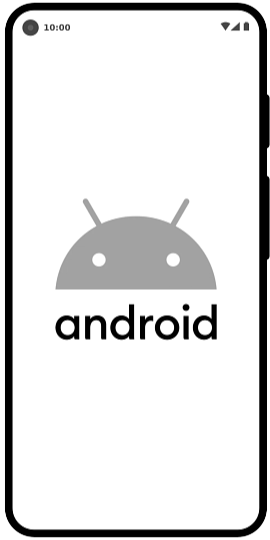
\includegraphics[height=0.5\textheight]{figures/android_device.png}
    \end{figure}
  \end{minipage}
\end{frame}


\section{Introduction}

\begin{frame}{Introduction}
  \begin{minipage}{0.49\textwidth} 
    \begin{itemize}
      \item Misuse of the Android API
      \pause
      \item Used for targeted advertisements
      \pause
      \item Does not require user permission
    \end{itemize}
  \end{minipage}
  \hfill
  \begin{minipage}{0.49\textwidth} 
    \begin{figure}
      \centering
      
\includegraphics[height=0.5\textheight]{figures/fingerprint.png}
    \end{figure}
  \end{minipage}
\end{frame}


\section{Background}

\begin{frame}{Browser Fingerprinting Methodologies}
  \begin{minipage}{0.49\textwidth} 
    \begin{itemize}
      \item Analyzing various browser-specific attributes
      \pause
      \item Can be used to distinguish users across sessions
    \end{itemize}
  \end{minipage}
  \hfill
  \begin{minipage}{0.49\textwidth} 
    \begin{figure}
      \centering
      
\includegraphics[height=0.5\textheight]{figures/browser.png}
    \end{figure}
  \end{minipage}
\end{frame}

\begin{frame}{Browser Fingerprinting Protections}
  \begin{minipage}{0.49\textwidth} 
    \begin{itemize}
      \item Blocking the execution of JavaScript
      \pause
      \item Introduction of controlled randomization
    \end{itemize}
  \end{minipage}
  \hfill
  \begin{minipage}{0.49\textwidth} 
    \begin{figure}
      \centering
      
\includegraphics[height=0.5\textheight]{figures/jshelter.png}
      \caption{JShelter}
    \end{figure}
  \end{minipage}
\end{frame}

\begin{frame}{Smartphone Fingerprinting}
  \begin{minipage}{0.49\textwidth} 
    \begin{itemize}
      \item Zero permission identifiers
      \item Personalized configurations
    \end{itemize}
  \end{minipage}
  \hfill
  \begin{minipage}{0.49\textwidth} 
    \begin{figure}
      \centering
      
\includegraphics[height=0.5\textheight]{figures/machine.png}
    \end{figure}
  \end{minipage}
\end{frame}


\section{Sensor Fingerprinting}

\begin{frame}{Fingerprinting Sensors}
  \begin{minipage}{0.49\textwidth} 
    \begin{itemize}
      \item Measurement inaccuracy of sensors
      \item Simple to fingerprint via machine learning algorithmus
      \item Is constant over the sensors lifetime
    \end{itemize}
  \end{minipage}
  \hfill
  \begin{minipage}{0.49\textwidth} 
    \begin{figure}
      \centering
      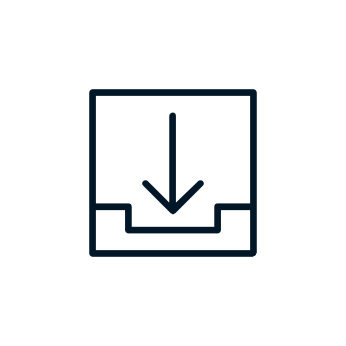
\includegraphics[height=0.5\textheight]{figures/download.png}
    \end{figure}
  \end{minipage}
\end{frame}


\section{Methodology}

\begin{frame}{Main Question}
  \begin{minipage}{0.525\textwidth} 
    How to protect against\\sensor fingerprinting
  \end{minipage}
  \hfill
  \begin{minipage}{0.455\textwidth} 
    \begin{figure}
      \centering
      
\includegraphics[height=0.5\textheight]{figures/question.png}
    \end{figure}
  \end{minipage}
\end{frame}

\begin{frame}<1>[label=props_sols]{Proposed Solutions}
  \begin{minipage}{0.49\textwidth} 
    \begin{itemize}
      \item<1> Calibration
      \item<2> Noise Generation
    \end{itemize}
  \end{minipage}
  \hfill
  \begin{minipage}{0.49\textwidth} 
    \begin{figure}
      \centering
      
\includegraphics[height=0.5\textheight]{figures/light-bulb.png}
    \end{figure}
  \end{minipage}
\end{frame}

\begin{frame}{Calibration}
  \begin{minipage}{0.49\textwidth} 
    \begin{itemize}
      \item Systematic adjustment of sensor readings
      \item Correcting the sensor data
    \end{itemize}
  \end{minipage}
  \hfill
  \begin{minipage}{0.49\textwidth} 
    \begin{figure}
      \centering
      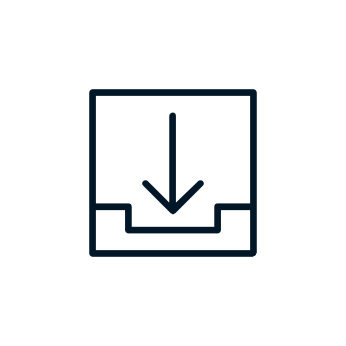
\includegraphics[height=0.5\textheight]{figures/download.png}
    \end{figure}
  \end{minipage}
\end{frame}

\againframe<2->{props_sols}

\begin{frame}{Noise Generation}
  \begin{minipage}{0.49\textwidth} 
    \begin{itemize}
      \item Introduces variability into the sensor data
      \item Masks the original values
    \end{itemize}
  \end{minipage}
  \hfill
  \begin{minipage}{0.49\textwidth} 
    \begin{figure}
      \centering
      
\includegraphics[height=0.5\textheight]{figures/noise.png}
    \end{figure}
  \end{minipage}
\end{frame}

\begin{frame}<1>[label=props_challs]{Challenges}
  \begin{minipage}{0.49\textwidth} 
    \begin{itemize}
      \item<1> Calibration
      \item<2> Noise Generation
    \end{itemize}
  \end{minipage}
  \hfill
  \begin{minipage}{0.49\textwidth} 
    \begin{figure}
      \centering
      
\includegraphics[height=0.5\textheight]{figures/exclamation.png}
    \end{figure}
  \end{minipage}
\end{frame}

\begin{frame}{Calibration}
  \begin{minipage}{0.49\textwidth} 
    \begin{itemize}
      \item Requires user awareness and interaction
      \item Requires precision
    \end{itemize}
  \end{minipage}
  \hfill
  \begin{minipage}{0.49\textwidth} 
    \begin{figure}
      \centering
      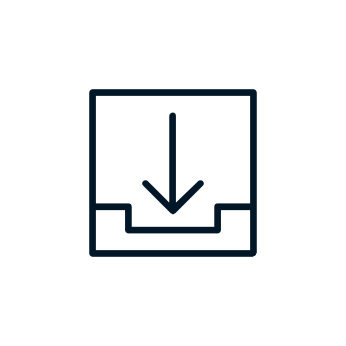
\includegraphics[height=0.5\textheight]{figures/download.png}
    \end{figure}
  \end{minipage}
\end{frame}

\againframe<2->{props_challs}

\begin{frame}{Noise Generation}
  \begin{minipage}{0.49\textwidth} 
    \begin{itemize}
      \item Degrade the functionality of applications
      \item Code has to be modified
    \end{itemize}
  \end{minipage}
  \hfill
  \begin{minipage}{0.49\textwidth} 
    \begin{figure}
      \centering
      
\includegraphics[height=0.5\textheight]{figures/noise.png}
    \end{figure}
  \end{minipage}
\end{frame}

\section{Approach}

\begin{frame}{Our Methodology}
  \begin{minipage}{0.49\textwidth} 
    \begin{itemize}
      \item Noise Generation
      \item Patch application vie A2P2 framework
    \end{itemize}
  \end{minipage}
  \hfill
  \begin{minipage}{0.49\textwidth} 
    \begin{figure}
      \centering
      
\includegraphics[height=0.5\textheight]{figures/android.png}
    \end{figure}
  \end{minipage}
\end{frame}

\begin{frame}{Modifying the Sensor API}
  \begin{minipage}{0.49\textwidth} 
    \begin{itemize}
      \item Intercept calls to registerListener method
      \pause
      \item Provide modified values to onSensorChanged method
    \end{itemize}
  \end{minipage}
  \hfill
  \begin{minipage}{0.49\textwidth} 
    \begin{figure}
      \centering
      
\includegraphics[height=0.5\textheight]{figures/code.png}
    \end{figure}
  \end{minipage}
\end{frame}

\begin{frame}{Noise Generation}
  \begin{minipage}{0.49\textwidth} 
    \begin{itemize}
      \item Adds random gain and offset to every value
      \item masks values
    \end{itemize}
  \end{minipage}
  \hfill
  \begin{minipage}{0.49\textwidth} 
    \begin{figure}
      \centering
      
\includegraphics[height=0.5\textheight]{figures/noise.png}
    \end{figure}
  \end{minipage}
\end{frame}

\begin{frame}{Loss of Precision}
  \begin{minipage}{0.49\textwidth} 
    \begin{itemize}
      \item 
    \end{itemize}
  \end{minipage}
  \hfill
  \begin{minipage}{0.49\textwidth} 
    \begin{figure}
      \centering
      
\includegraphics[height=0.5\textheight]{figures/noise.png}
    \end{figure}
  \end{minipage}
\end{frame}

\section{Implementation}

\begin{frame}<1>[label=impl]{Implementation}
  \begin{minipage}{0.49\textwidth} 
    \begin{itemize}
      \item Intercept Method
      \pause
      \item Noise Generating Function
      \pause
      \item Random Value Generation Function
    \end{itemize}
  \end{minipage}
  \hfill
  \begin{minipage}{0.49\textwidth} 
    \begin{figure}
      \centering
      
\includegraphics[height=0.5\textheight]{figures/java.png}
    \end{figure}
  \end{minipage}
\end{frame}

\begin{frame}{Intercept Method}
  \begin{textblock*}{\textwidth}(30pt,50pt)
  \begin{figure}
    \centering
    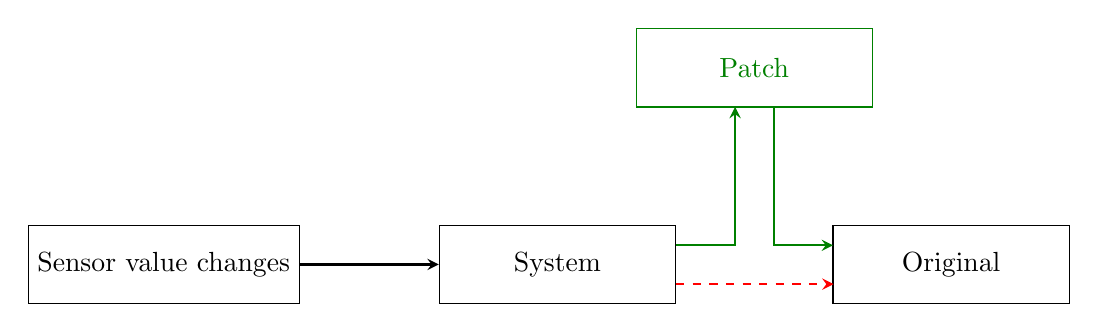
\begin{tikzpicture}
      \tikzstyle{process} = [rectangle, minimum width=3cm, minimum height=1cm, text centered, draw=black]

      \node (sensor) [process] at (0,0) {Sensor value changes};
      \node (system) [process] at (5,0) {System};
      \node (patch) [process, black!50!green] at (7.5,2.5) {Patch};
      \node (function) [process] at (10,0) {Original};

      \draw [thick, ->, >=stealth] (sensor) -- (system);
      \draw [thick, ->, >=stealth, red, dashed] (system.east)+(0,-0.25) -- +(2,-0.25);
      \draw [thick, ->, >=stealth, black!50!green] (system.east)+(0,0.25) -| +(0.75,2);
      \draw [thick, ->, >=stealth, black!50!green] (patch.south)+(0.25,0) |- +(1,-1.75);
    \end{tikzpicture}
    \caption{The function calls from the system are intercepted by our patch and forwarded after modification to the original function.}
  \end{figure}
  \end{textblock*}
\end{frame}

\againframe<2->{impl}

\begin{frame}{Application of Patch}
  \begin{minipage}{0.49\textwidth} 
    \begin{itemize}
      \item Intercept the original method
      \pause
      \item Apply appropriate random noise
      \pause
      \item Return obstructed sensor data to original method
    \end{itemize}
  \end{minipage}
  \hfill
  \begin{minipage}{0.49\textwidth} 
    \begin{figure}
      \centering
      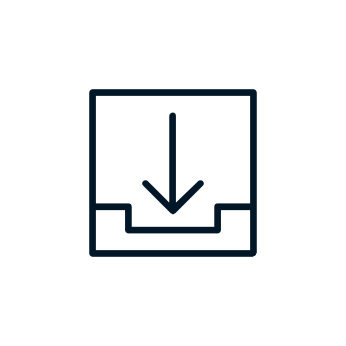
\includegraphics[height=0.5\textheight]{figures/download.png}
    \end{figure}
  \end{minipage}
\end{frame}

\section{Evaluation}

\begin{frame}{Testing}
  \begin{minipage}{0.49\textwidth} 
    \begin{itemize}
      \item Incorporates the patch into a valid APK
      \item Intercepts the original function calls
      \item Executes the patch
    \end{itemize}
  \end{minipage}
  \hfill
  \begin{minipage}{0.49\textwidth} 
    \begin{figure}
      \centering
      
\includegraphics[height=0.5\textheight]{figures/code.png}
    \end{figure}
  \end{minipage}
\end{frame}

\begin{frame}{Functionality}
  \begin{minipage}{0.49\textwidth} 
    \begin{itemize}
      \item Incorporates the patch into a valid APK
      \item Intercepts the original function calls
      \item Executes the patch
    \end{itemize}
  \end{minipage}
  \hfill
  \begin{minipage}{0.49\textwidth} 
    \begin{figure}
      \centering
      
\includegraphics[height=0.5\textheight]{figures/code.png}
    \end{figure}
  \end{minipage}
\end{frame}

\begin{frame}{Effectiveness}
  \begin{minipage}{0.49\textwidth}
    \begin{figure}
      \centering
      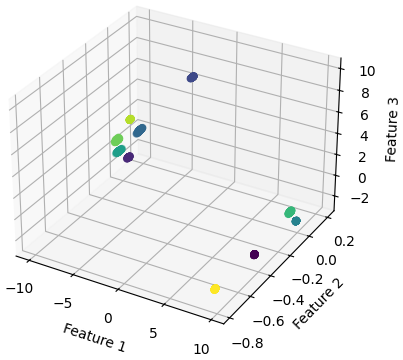
\includegraphics[height=0.65\textheight]{figures/knn_before.png}
    \end{figure}
  \end{minipage}
  \hfill
  \begin{minipage}{0.49\textwidth}
    \begin{figure}
      \centering
      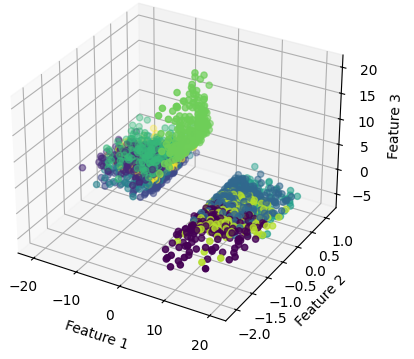
\includegraphics[height=0.65\textheight]{figures/knn_after.png}
    \end{figure}
  \end{minipage}
\end{frame}

\begin{frame}{Usability}
  \begin{minipage}{0.49\textwidth} 
    \begin{itemize}
      \item Incorporates the patch into a valid APK
      \item Intercepts the original function calls
      \item Executes the patch
    \end{itemize}
  \end{minipage}
  \hfill
  \begin{minipage}{0.49\textwidth} 
    \begin{figure}
      \centering
      
\includegraphics[height=0.5\textheight]{figures/code.png}
    \end{figure}
  \end{minipage}
\end{frame}

\begin{frame}{Noise Level Adjustment}
  \begin{minipage}{0.49\textwidth} 
    \begin{itemize}
      \item Incorporates the patch into a valid APK
      \item Intercepts the original function calls
      \item Executes the patch
    \end{itemize}
  \end{minipage}
  \hfill
  \begin{minipage}{0.49\textwidth} 
    \begin{figure}
      \centering
      
\includegraphics[height=0.5\textheight]{figures/noise.png}
    \end{figure}
  \end{minipage}
\end{frame}

\section{Discussion \& Limitations}

\begin{frame}{Discussion \& Limitations}
  \begin{minipage}{0.49\textwidth} 
    \begin{itemize}
      \item Comparing values before and after the patch
      \item Could not be done sufficiently due to limited access to supported hardware
    \end{itemize}
  \end{minipage}
  \hfill
  \begin{minipage}{0.49\textwidth} 
    \begin{figure}
      \centering
      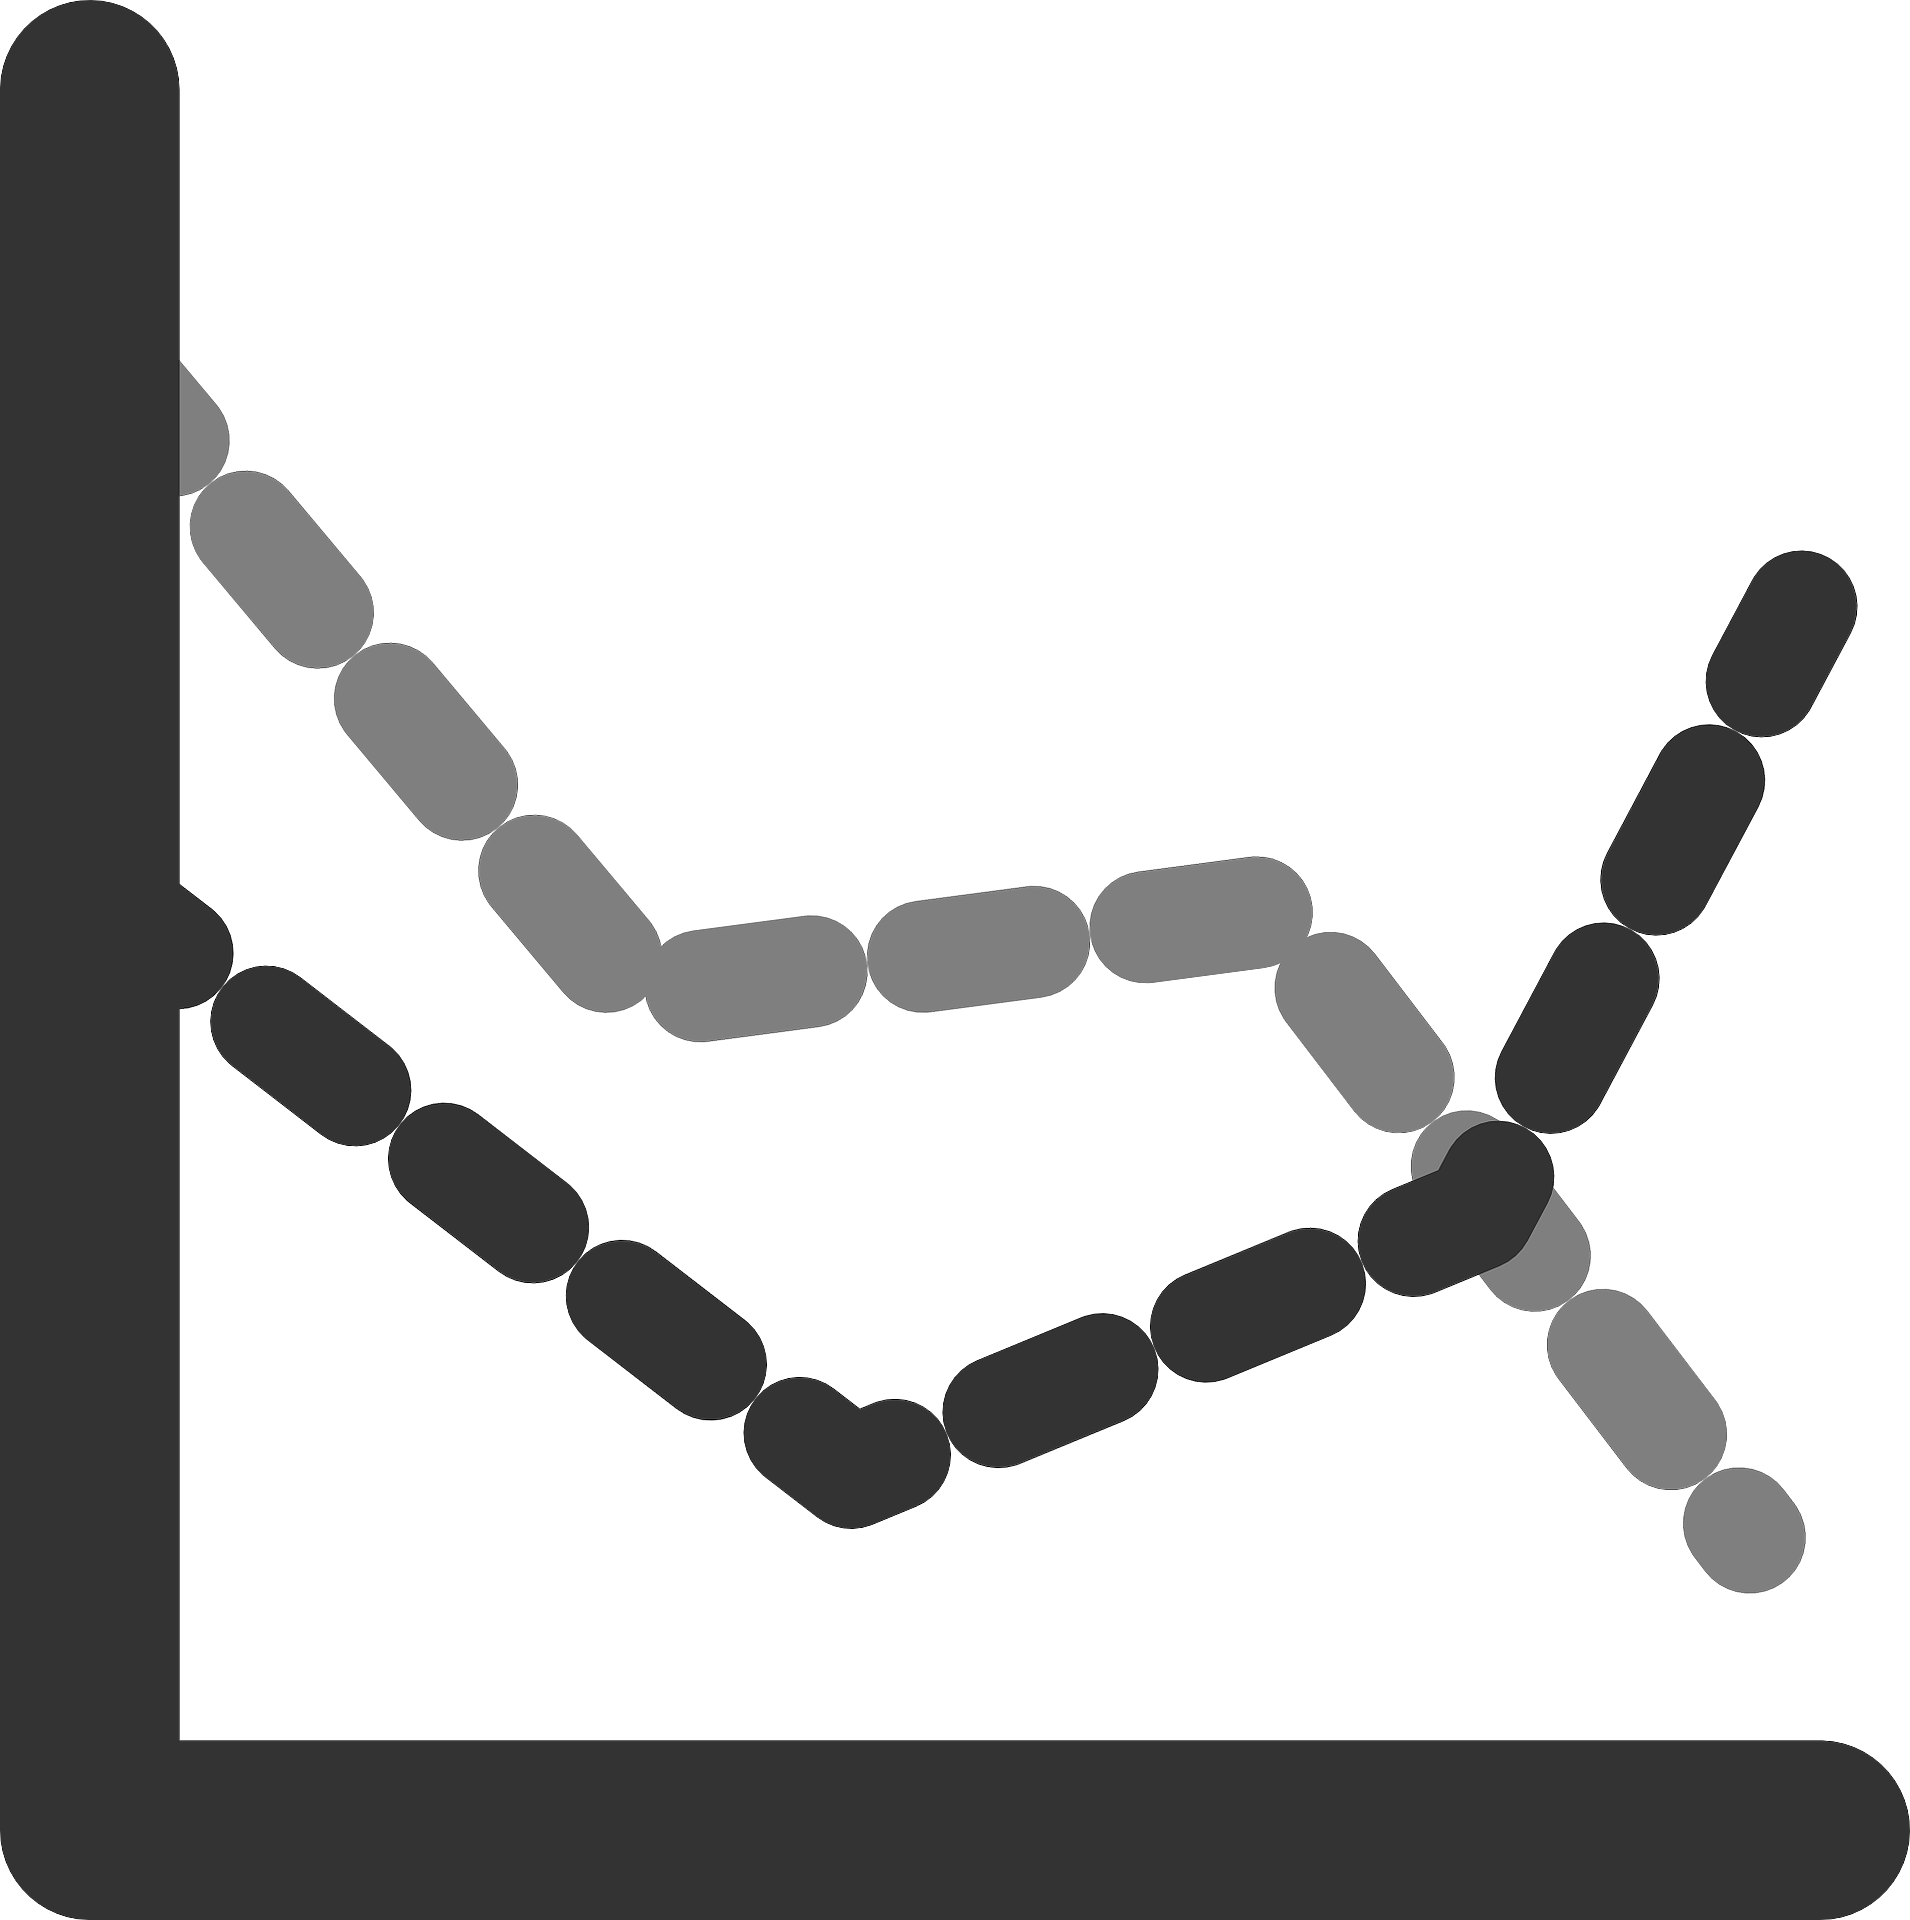
\includegraphics[height=0.5\textheight]{figures/graph.png}
    \end{figure}
  \end{minipage}
\end{frame}

\section*{}

\begin{frame}{Conclusion}
  \begin{minipage}{0.49\textwidth} 
    \begin{itemize}
      \item Masking the sensor values decreases fingerprintability
      \item Modifying the SensorEventListener makes it easy to incorporate the patch into the Android API
    \end{itemize}
  \end{minipage}
  \hfill
  \begin{minipage}{0.49\textwidth} 
    \begin{figure}
      \centering
      
\includegraphics[height=0.5\textheight]{figures/androguard.png}
    \end{figure}
  \end{minipage}
\end{frame}


% \begin{frame}{Bibliography}
%   ...
% \end{frame}

\end{document}
